%======================================================================
\chapter{Tree-like continua}\label{ch:tree}
%======================================================================

A continuum is \emph{tree-like} if it can be covered by arbitrarily fine tree chains: finite
coherent collections of open sets with no triple points and no circular subchains. This chapter
proves R.~H.~Bing's characterization of tree-like plane continua:

\begin{quote}
A plane continuum is tree-like if and only if none of its subcontinua separates the plane.
\end{quote}

The direction ``tree-like $\Rightarrow$ no separating subcontinuum'' is proved with logarithms: on a
fine tree chain far from a point $p$, the function $z-p$ has a logarithm, which a separating
continuum around $p$ cannot carry (Theorem~\ref{thm:treelike-nonsep}). The direction ``no separating
subcontinuum $\Rightarrow$ tree-like'' is Bing's Theorem~6 (Theorem~\ref{thm:bing6}); the proof given
here combines the notched-square covers of Bing with the enclosing polygons of
Chapter~\ref{ch:enc} and the compact form of Janiszewski's theorem (Theorem~\ref{thm:janiszewski}).
On tree-like continua every nonvanishing function has a logarithm
(Theorem~\ref{thm:log-treelike}), and this gives a weak form of the topological invariance of plane
separation which does not depend on Borsuk's theorem (Section~\ref{sec:weak-invariance}). The
chapter ends with a survey of Bing's Theorem~7, which refines the links of the tree chains to
interiors of polygons.

Throughout, ``continuum'' means a nonempty compact connected subset of $\R^2$.

\section{Tree chains}

\begin{definition}\label{def:treechain}
Let $G$ be a finite collection of subsets of $\R^2$ (the \emph{links}).
\begin{itemize}
\item $G$ is \emph{coherent} if for every nonempty proper subcollection $G'\subsetneq G$ some link of
$G'$ meets some link of $G\setminus G'$.
\item $G$ is a \emph{circular chain} if it consists of $m\ge3$ distinct links
$d_0,\dots,d_{m-1}$ such that $d_i\cap d_j\neq\emptyset$ if and only if $\abs{i-j}\le1$ or
$\set{i,j}=\set{0,m-1}$.
\item $G$ is a \emph{tree chain} if its links are open, $G$ is coherent, no three distinct links
have a common point, and no subcollection of $G$ is a circular chain.
\end{itemize}
A continuum $M$ is \emph{tree-like} if for every $\varepsilon>0$ there is a tree chain $G$ covering
$M$ whose links are bounded and of diameter less than $\varepsilon$.
\end{definition}

\formal{\lean{HPC.Plane.IsCoherent}, \lean{HPC.Plane.IsCircularChain}, \lean{HPC.Plane.IsTreeChain},
\lean{HPC.Plane.IsTreeLike}.}

The circular chains here are the circular chains of \vthree{Definition~5.13}, without the bound on
the mesh. Note the case $m=3$: \emph{three distinct pairwise meeting sets form a circular chain}, since
for $m=3$ every pair of indices satisfies the condition. So in a tree chain no three links meet
pairwise, even without a common point.

\begin{remark}[Bounded links]
The links of the tree chains in the definition of tree-likeness are required to be bounded. In the
formal development the diameter of an unbounded set is $0$ (a convention of Mathlib), so without
this requirement the one-link collection $\set{\R^2}$ would be a tree chain of every mesh, and every
continuum, a circle included, would be tree-like. An early version of the definition had exactly
this defect; it is kept, with the proof that it is satisfied by every continuum, as a warning.
(\lean{HPC.Plane.IsTreeLikeOld}, \lean{HPC.Plane.isTreeChain_univ},
\lean{HPC.Plane.isTreeLikeOld_of_isContinuum}.)
\end{remark}

\begin{lemma}\label{lem:coherent-cover}
Let $M$ be connected and $G$ a finite collection of open sets covering $M$, each of which meets $M$.
Then $G$ is coherent.
\end{lemma}

\begin{proof}
If $G'\subsetneq G$ is nonempty and no link of $G'$ meets a link of $G\setminus G'$, the open sets
$\bigcup G'$ and $\bigcup(G\setminus G')$ are disjoint, cover $M$, and both meet $M$; this
contradicts the connectedness of $M$.
\end{proof}

\formal{\lean{HPC.Plane.isCoherent_of_minimal_cover}.}

\begin{lemma}\label{lem:filter-meet}
Let $G$ be a tree chain and $K\subseteq\bigcup G$ connected. The links of $G$ that meet $K$ form a tree
chain.
\end{lemma}

\begin{proof}
Openness, the absence of triple points and of circular subchains pass to subcollections; coherence
is Lemma~\ref{lem:coherent-cover} applied to $K$.
\end{proof}

\formal{\lean{HPC.Plane.isTreeChain_filter_meet}.}

The next lemma says that the nerve of a tree chain is a tree, in the form needed for inductions: a
tree chain has a leaf.

\begin{lemma}[Leaves]\label{lem:leaf}
Let $G$ be a tree chain with at least two links. There are distinct links $A,B\in G$ such that $A$
meets $B$, $A$ is disjoint from every other link of $G$, and $G\setminus\set A$ is a tree chain.
\end{lemma}

\begin{proof}
Call a subcollection $H\subseteq G$ \emph{chain-connected} if any two links of $H$ are joined by a
sequence of links of $H$, consecutive ones meeting. A chain-connected collection is coherent (a
sequence from a link of $H'$ to a link of $H\setminus H'$ has two consecutive links on different
sides). Conversely, starting from one link and adding, at each step, a link of $G$ meeting one of the
links already chosen (it exists by the coherence of $G$), we obtain chain-connected subcollections of
$G$ of every size; let $H$ be one with all links but one, $G\setminus H=\set C$.

By coherence, $C$ meets some link $B$ of $H$. Suppose $C$ meets two distinct links of $H$. Among all
pairs of distinct links $X,Y\in H$ meeting $C$ and all sequences $X=P_0,P_1,\dots,P_k=Y$ of links of
$H$ with consecutive links meeting, choose one with $k$ minimal; then $k\ge1$. By minimality, no
inner link $P_1,\dots,P_{k-1}$ meets $C$ (it would give a shorter pair), and $P_i\cap P_j=\emptyset$
for $\abs{i-j}\ge2$ (a shortcut would give a shorter sequence); the links $P_i$ are distinct for the
same reason. So $C,P_0,\dots,P_k$ is a circular chain of $k+2\ge3$ links (for $k=1$, three pairwise
meeting links), contradicting the definition of a tree chain. Hence $C$ meets exactly one link $B$ of
$H$, and $A=C$ is the required leaf: $G\setminus\set A=H$ is coherent, and the other conditions pass to
subcollections.
\end{proof}

\formal{\lean{HPC.Plane.exists_leaf}, from \lean{HPC.Plane.ChainConn},
\lean{HPC.Plane.isCoherent_of_chainConn}, \lean{HPC.Plane.exists_chainConn_card},
\lean{HPC.Plane.circularChain_of_minimal} and \lean{HPC.Plane.no_two_nbrs}.}

\section{Tree-like continua do not contain separating continua}

\begin{theorem}[A logarithm on a fine tree chain]\label{thm:log-treechain}
Let $\varepsilon>0$, $p\in\R^2$, and let $G$ be a tree chain whose links are bounded, of diameter
less than $\varepsilon$, and consist of points at distance more than $8\varepsilon$ from $p$. Then
$z\mapsto z-p$ has a logarithm on $\bigcup G$.
\end{theorem}

\begin{proof}
We prove, by induction on the number of links, the stronger statement: \emph{there is a function $L$
such that for every nonempty link $A$ there are a ball $B(c,\varepsilon)\supseteq A$ and a logarithm
$\ell$ of $z-p$ on $B(c,\varepsilon)$ with $L=\ell$ on $A$.} This implies the theorem: the links are
open, so $L$ coincides near each point of $\bigcup G$ with a continuous function.

For a single nonempty link $A$ pick $a\in A$; then $A\subseteq B(a,\varepsilon)$ since $\diam
A<\varepsilon$, and since $d(a,p)>8\varepsilon>4\varepsilon$, Lemma~\ref{lem:log-ball} gives a
logarithm on $B(a,\varepsilon)$.

For the inductive step let $A,B$ be as in Lemma~\ref{lem:leaf} and let $L_0$ be given by the induction
hypothesis for $G\setminus\set A$, with ball $B(c_B,\varepsilon)$ and logarithm $\ell_B$ for the link
$B$. As above, $A$ lies in a ball $B(c_A,\varepsilon)$ carrying a logarithm $\ell_A$. The intersection
$S=B(c_A,\varepsilon)\cap B(c_B,\varepsilon)$ is convex and contains a point $z_0\in A\cap B$, so
$\ell_B-\ell_A$ is a constant $\kappa$ on $S$, with $e^\kappa=1$ (Lemma~\ref{lem:log-unique}). Define
$L=\ell_A+\kappa$ on $A$ and $L=L_0$ elsewhere. On $A$ the invariant holds with the logarithm
$\ell_A+\kappa$. On $B$ it holds with $\ell_B$: on $B\setminus A$ by the choice of $L_0$, and on
$A\cap B\subseteq S$ because $\ell_A+\kappa=\ell_B$ there. The other links are disjoint from $A$.
\end{proof}

\formal{\lean{HPC.Plane.exists_log_on_treeChain}, by induction (\lean{HPC.Plane.exists_log_inv}) with
\lean{HPC.Plane.exists_ball_branch}.}

The balls are what makes the induction work: the intersection $A\cap B$ of two links need not be
connected, so two logarithms which agree at one point of $A\cap B$ need not agree on all of it; on
the convex set $S\supseteq A\cap B$ they do.

\begin{theorem}\label{thm:treelike-nonsep}
A tree-like continuum $M$ contains no continuum that separates the plane.
\end{theorem}

\begin{proof}
Let $K\subseteq M$ be a continuum separating the plane. By Lemma~\ref{lem:unbounded-comp}(b) there is
$p\notin K$ with $\comp Kp$ bounded. Let $d=\dist(p,K)>0$ and $\varepsilon=d/10$. Take a tree chain $G$
of bounded links of diameter $<\varepsilon$ covering $M$, and let $G'$ be the collection of its links
meeting $K$, a tree chain covering $K$ (Lemma~\ref{lem:filter-meet}). A point $z$ of a link of $G'$
is within $\varepsilon$ of a point of $K$, so $d(z,p)>d-\varepsilon=9\varepsilon>8\varepsilon$. By
Theorem~\ref{thm:log-treechain}, $z-p$ has a logarithm on $W=\bigcup G'$.

$W$ is open, $p\notin W$ and $K\subseteq W$, so the component of $p$ in $\R^2\setminus W$ lies in
$\comp Kp$ and is bounded. By Theorem~\ref{thm:polygon-around} there is a simple closed polygon
$J\subseteq W$ with $p\in\inn J$; the logarithm on $W$ restricts to one on $J$, contradicting
Theorem~\ref{thm:nolog-polygon}.
\end{proof}

\formal{\lean{HPC.Plane.treeLike_nonseparating}.}

\begin{remark}
The last paragraph can be replaced by a reference to Corollary~\ref{cor:nolog-bounded}: the
logarithm on $W$ restricts to a logarithm of $z-p$ on $K$, and there is none since $\comp Kp$ is
bounded. The formal proof uses the polygon, which was available earlier in the development; both
arguments are complete.
\end{remark}

\section{Logarithms on tree-like continua}

On a tree-like continuum every nonvanishing function has a logarithm. The proof is a variant of
that of Theorem~\ref{thm:log-treechain} in which the branches are centred at points of the continuum,
so that no balls are needed.

\begin{theorem}\label{thm:log-treelike}
Let $K$ be a tree-like continuum and $f$ continuous and nowhere zero on $K$. Then $f$ has a logarithm
on $K$.
\end{theorem}

\begin{proof}
Let $m=\min_K\abs f>0$ and, by uniform continuity, $\delta>0$ with $\abs{f(x)-f(y)}<m/2$ for $x,y\in K$,
$d(x,y)<\delta$. For such $x,y$ we have $\abs{f(x)/f(y)-1}<\frac12$. For $a\in K$ the \emph{branch
centred at $a$} is
\[
b_a(z)=\Log\frac{f(z)}{f(a)}+\Log f(a);
\]
it is continuous on $\set{z\in K:d(z,a)<\delta}$, with $e^{b_a}=f$ there.

\emph{Overlaps.} Let $a,b,z\in K$ with $d(b,a)<\delta$ and $d(z,b)<\delta$. Then
$\frac{f(z)}{f(a)}=\frac{f(z)}{f(b)}\cdot\frac{f(b)}{f(a)}$ with both factors within $\frac12$ of $1$, so
$\Log$ is additive on them (Section~\ref{sec:log-unique}) and
\[
b_b(z)-b_a(z)=\Log f(b)-\Log f(a)-\Log\frac{f(b)}{f(a)}=:\kappa_{ab},
\]
a constant independent of $z$, with $e^{\kappa_{ab}}=1$.

\emph{Gluing.} Take a tree chain of bounded links of diameter $<\delta/2$ covering $K$, and keep the
links meeting $K$; this is a tree chain $G$ (Lemma~\ref{lem:filter-meet}). By induction on the number
of links we find $L$ such that for every $A\in G$ there are $a\in A\cap K$ and $\kappa_A$ with
$e^{\kappa_A}=1$ and $L=b_a+\kappa_A$ on $A\cap K$. For the inductive step take a leaf $A$ with
neighbour $B$ (Lemma~\ref{lem:leaf}), $L_0$ for $G\setminus\set A$ with centre $b\in B\cap K$ and
constant $\kappa_B$, and any $a\in A\cap K$. Since $A$ and $B$ meet and have diameter $<\delta/2$, we have
$d(b,a)<\delta$, and $d(z,b)<\delta$ for $z\in A\cap B$. Put $L=b_a+\kappa_{ab}+\kappa_B$ on $A\cap K$ and
$L=L_0$ elsewhere; by the overlap formula it agrees with $b_b+\kappa_B=L_0$ on $A\cap B\cap K$, and
the other links miss $A$.

Each point of $K$ lies in an open link $A$, on which $L$ is a continuous branch plus a constant, and
$e^L=e^{b_a}=f$ there.
\end{proof}

\formal{\lean{HPC.Hagopian.exists_log_of_isTreeLike}, from \lean{HPC.Hagopian.branchAt},
\lean{HPC.Hagopian.LogData}, \lean{HPC.Hagopian.LogData.branch_sub},
\lean{HPC.Hagopian.LogData.exp_const}, \lean{HPC.Hagopian.LogData.exists_glue} and
\lean{HPC.Hagopian.log_mul_near_one}.}

Together with Theorem~\ref{thm:bing6} below, Theorem~\ref{thm:log-treelike} is a form of Borsuk's
theorem (Theorem~\ref{thm:borsuk}) for continua none of whose subcontinua separates the plane, proved
without the smoothing and regular values of Chapter~\ref{ch:sep}.

\section{Bing's Theorem 6}

\begin{theorem}[Bing]\label{thm:bing6}
A continuum $M$ no subcontinuum of which separates the plane is tree-like.
\end{theorem}

The proof occupies this section. Fix $M$ and $\varepsilon>0$; we construct a tree chain of mesh less
than $\varepsilon$ covering $M$, in four steps: a cover of $M$ by \emph{notched squares} without triple
points; an enclosing polygon $J$ inside this cover; the components of the sets $\inn J\cap d$ as
links; and the proof that they contain no circular chain.

\subsection*{Step 1: notched squares}

\begin{lemma}\label{lem:no-interior}
If no subcontinuum of $M$ separates the plane, $M$ has empty interior.
\end{lemma}

\begin{proof}
If $B(x,r)\subseteq M$, then $M$ contains the sphere $\set{z:d(z,x)=r/2}$, the boundary of a square,
which is a continuum separating $x$ from $x+(r,r)$.
\end{proof}

\formal{\lean{HPC.Plane.interior_eq_empty_of_noSeparating}.}

Fix $\delta>0$. For an offset $o\in\R^2$ and $a,b\in\Z$ let
$Q_{ab}=[o_1+\delta a,o_1+\delta(a+1)]\times[o_2+\delta b,o_2+\delta(b+1)]$ be the grid squares, with
the points $(o_1+\delta a,o_2+\delta b)$ as \emph{grid vertices}.

\begin{lemma}[Bing's offset]\label{lem:offset}
Let $M$ be closed with empty interior. Some offset $o$ puts no grid vertex on $M$.
\end{lemma}

\begin{proof}
The offsets that put the vertex with index $(a,b)$ on $M$ form the translate $M-(\delta a,\delta b)$,
a closed set with empty interior. By Baire's theorem countably many such sets do not cover $\R^2$.
\end{proof}

\formal{\lean{HPC.Plane.gridSq}, \lean{HPC.Plane.gridVertices}, \lean{HPC.Plane.exists_grid_offset}.}

For $0<\eta<r$ the \emph{notched square} $N_{ab}$ is the open square $\interior Q_{ab}$ together with
four open strips of width $\eta$ along the outside of its sides, each stopped at distance $r$ from the
two ends of its side:
\[
N_{ab}=\interior Q_{ab}\;\cup\;(x_a+r,\,x_{a+1}-r)\times(y_b-\eta,\,y_{b+1}+\eta)\;\cup\;
(x_a-\eta,\,x_{a+1}+\eta)\times(y_b+r,\,y_{b+1}-r),
\]
where $x_a=o_1+\delta a$ and $y_b=o_2+\delta b$.

\begin{center}
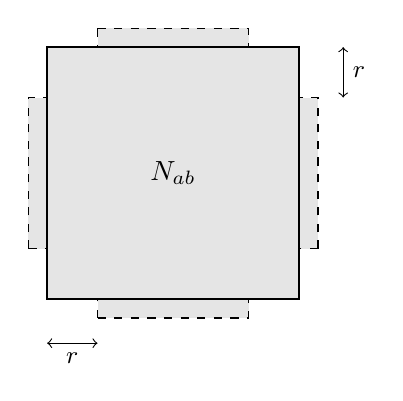
\begin{tikzpicture}[scale=1.6]
\fill[gray!20] (0,0) rectangle (2,2);
\fill[gray!20] (0.4,-0.15) rectangle (1.6,2.15);
\fill[gray!20] (-0.15,0.4) rectangle (2.15,1.6);
\draw[thick] (0,0) rectangle (2,2);
\draw[dashed] (0.4,-0.15) -- (1.6,-0.15) -- (1.6,0);
\draw[dashed] (0.4,-0.15) -- (0.4,0);
\draw[dashed] (0.4,2.15) -- (1.6,2.15) -- (1.6,2);
\draw[dashed] (0.4,2.15) -- (0.4,2);
\draw[dashed] (-0.15,0.4) -- (-0.15,1.6) -- (0,1.6);
\draw[dashed] (-0.15,0.4) -- (0,0.4);
\draw[dashed] (2.15,0.4) -- (2.15,1.6) -- (2,1.6);
\draw[dashed] (2.15,0.4) -- (2,0.4);
\node at (1,1) {$N_{ab}$};
\draw[<->] (0,-0.35) -- (0.4,-0.35) node[midway,below] {\small $r$};
\draw[<->] (2.35,1.6) -- (2.35,2) node[midway,right] {\small $r$};
\end{tikzpicture}
\end{center}

\begin{lemma}\label{lem:notched}
Let $0<\eta<r$ with $2r<\delta$.
\begin{enumerate}[label=(\alph*)]
\item $N_{ab}$ is open, bounded, and $\diam N_{ab}\le\delta+2\eta$.
\item If $M$ has distance more than $r$ from every grid vertex, then $M\cap Q_{ab}\subseteq N_{ab}$.
Hence the notched squares of the finitely many grid squares meeting $M$ cover $M$.
\item $N_{ab}$ and $N_{a+1,b+1}$ are disjoint, and so are $N_{a+1,b}$ and $N_{a,b+1}$. Two notched
squares meet only if their grid squares coincide or share a side.
\item No three distinct notched squares have a common point.
\end{enumerate}
\end{lemma}

\begin{proof}
(a) is clear (sup metric). (b) A point of $M\cap Q_{ab}$ not in the open square lies on a side, at
distance more than $r$ from both ends of it (they are grid vertices); so it lies in the strip along
that side. (c) Write $c=(x_{a+1},y_{b+1})$ for the common corner of $Q_{ab}$ and $Q_{a+1,b+1}$. A
point $z$ of $N_{ab}$ has $z_1<x_{a+1}+\eta$, $z_2<y_{b+1}+\eta$, and $z_2<y_{b+1}-r$ if $z_1\ge x_{a+1}$. A
point $z$ of $N_{a+1,b+1}$ has $z_1>x_{a+1}+r$ if $z_2\le y_{b+1}$, and $z_2>y_{b+1}+r$ if $z_1\le x_{a+1}$.
For a common point, if $z_1\ge x_{a+1}$ then $z_2<y_{b+1}$, so $z_1>x_{a+1}+r>x_{a+1}+\eta$, which is
impossible; if $z_1<x_{a+1}$ then $z_2>y_{b+1}+r>y_{b+1}+\eta$, also impossible. The other pair is
symmetric. A point common to two notched squares is within $\eta<\delta/2$ of both squares,
so their indices differ by at most one in each coordinate; by the first part they are not diagonal
neighbours. (d) Three distinct grid squares cannot pairwise coincide or share a side: two of them would
be diagonal neighbours.
\end{proof}

\formal{\lean{HPC.Plane.notched}, \lean{HPC.Plane.isOpen_notched}, \lean{HPC.Plane.diam_notched_le},
\lean{HPC.Plane.inter_gridSq_subset_notched}, \lean{HPC.Plane.notched_diag1},
\lean{HPC.Plane.notched_diag2}, \lean{HPC.Plane.notched_adj}, \lean{HPC.Plane.notched_no_triple}.}

\begin{corollary}\label{cor:notched-cover}
If no subcontinuum of $M$ separates the plane and $\varepsilon>0$, there is a finite collection $D$ of
bounded open sets of diameter $<\varepsilon$ covering $M$, no three of which have a common point.
\end{corollary}

\begin{proof}
Let $\delta=\varepsilon/2$. By Lemmas~\ref{lem:no-interior} and~\ref{lem:offset} choose an offset with
no grid vertex on $M$; the grid vertices form a closed set, so they have distance $r_0>0$ from the
compact set $M$. Put $r=\min(r_0/2,\delta/4)$, $\eta=r/2$, and apply Lemma~\ref{lem:notched}: the
diameters are at most $\delta+2\eta\le\frac54\delta<\varepsilon$.
\end{proof}

\formal{\lean{HPC.Plane.exists_far}, \lean{HPC.Plane.exists_notched_cover_bdd}.}

\subsection*{Step 2: the enclosing polygon, and the links}

Let $D$ be as in Corollary~\ref{cor:notched-cover}. Since $M$ does not separate the plane,
Theorem~\ref{thm:enclose} gives a simple closed polygon $J$ with $M\subseteq\inn J\subseteq\bigcup D$.
Let $\mathcal F$ be the family of all components of the sets $\inn J\cap d$, $d\in D$.

\begin{lemma}\label{lem:compfamily}
\begin{enumerate}[label=(\alph*)]
\item Every member of $\mathcal F$ is open, connected, contained in $\inn J$, and contained in a member
of $D$; so it is bounded, of diameter $<\varepsilon$.
\item Two meeting components of the same set $\inn J\cap d$ are equal.
\item No three distinct members of $\mathcal F$ have a common point.
\end{enumerate}
\end{lemma}

\begin{proof}
(a) Components of open sets of the plane are open (Lemma~\ref{lem:frontier-component}). (b) is a
property of components. (c) If $h_1,h_2,h_3\in\mathcal F$ are distinct with a common point, and $h_i$
is a component of $\inn J\cap d_i$, then by (b) the $d_i$ are distinct, and they have a common point.
\end{proof}

\formal{\lean{HPC.Plane.compFamily}, \lean{HPC.Plane.compFamily_props},
\lean{HPC.Plane.connectedComponentIn_eq_of_meet}, \lean{HPC.Plane.compFamily_no_triple}.}

\begin{lemma}\label{lem:cover-links}
Finitely many members of $\mathcal F$, each meeting $M$, cover $M$; any such collection $G$ is
coherent, has no triple points, and has bounded links of diameter $<\varepsilon$.
\end{lemma}

\begin{proof}
Each $x\in M$ lies in some $d\in D$ and in $\inn J$, hence in the component of $x$ in $\inn J\cap d$.
These components are open and cover the compact set $M$; take a finite subcover. Coherence is
Lemma~\ref{lem:coherent-cover}, the rest is Lemma~\ref{lem:compfamily}.
\end{proof}

It remains to show that no subcollection of $\mathcal F$ is a circular chain.

\subsection*{Step 3: a polygon through three sets}

\begin{lemma}[A theta polygon]\label{lem:theta-polygon}
Let $A_0,A_1,A_2$ be connected open sets which meet pairwise and have no common point. There are a
simple closed polygon $\Gamma$, connected sets $\alpha_i\subseteq A_i$ with
$\Gamma=\alpha_0\cup\alpha_1\cup\alpha_2$, and points $q_1\in\alpha_0\cap\alpha_1$,
$q_2\in\alpha_1\cap\alpha_2$, $q_0\in\alpha_2\cap\alpha_0$.
\end{lemma}

\begin{proof}
Choose $p_1\in A_0\cap A_1$, $p_2\in A_1\cap A_2$, $p_0\in A_2\cap A_0$, and simple polygonal arcs
$\beta_0\subseteq A_0$ from $p_0$ to $p_1$, $\beta_1\subseteq A_1$ from $p_1$ to $p_2$ and
$\beta_2\subseteq A_2$ from $p_2$ to $p_0$ (Proposition~\ref{prop:polypath}). Write $\beta[u,v]$ for the
subarc of an arc $\beta$ between two of its points. Trim, using
Proposition~\ref{prop:polypath}(c) each time:
\begin{itemize}
\item let $q_1$ be the first point of $\beta_0$ (from $p_0$) on $\beta_1$, and $\alpha_0'=\beta_0[p_0,q_1]$;
\item let $q_2$ be the first point of $\beta_1[q_1,p_2]$ (from $q_1$) on $\beta_2$, and
$\alpha_1=\beta_1[q_1,q_2]$;
\item let $q_0$ be the first point of $\beta_2[q_2,p_0]$ (from $q_2$) on $\alpha_0'$ (which contains
$p_0$), and put $\alpha_2=\beta_2[q_2,q_0]$, $\alpha_0=\alpha_0'[q_0,q_1]$.
\end{itemize}
Then $\alpha_0\cap\alpha_1=\set{q_1}$, $\alpha_1\cap\alpha_2=\set{q_2}$, $\alpha_2\cap\alpha_0=\set{q_0}$ by
the choice of first points. The points $q_1\in A_0\cap A_1$, $q_2\in A_1\cap A_2$, $q_0\in A_2\cap A_0$
are distinct because $A_0\cap A_1\cap A_2=\emptyset$. By Lemma~\ref{lem:closed-chain} (with $m=3$),
$\Gamma=\alpha_0\cup\alpha_1\cup\alpha_2$ is a simple closed polygon.
\end{proof}

\formal{\lean{HPC.Plane.exists_theta_polygon} (proved as \lean{HPC.Plane.theta_polygon_of_three}).
The general threading of a circular chain of $m$ connected open sets, \lean{HPC.Plane.exists_threaded},
is not needed here.}

\subsection*{Step 4: Bing's point}

The following lemma is the heart of the proof. It is the only place where Janiszewski's theorem is
used.

\begin{lemma}[Bing's point]\label{lem:bing-point}
Let $\Gamma$ be a simple closed polygon, $\Gamma=\alpha_1\cup\alpha_2\cup\beta$ with $\alpha_1,\alpha_2,\beta$
connected, and $p_2\in\alpha_1\cap\alpha_2$, $p_3\in\alpha_2\cap\beta$, $p_1\in\beta\cap\alpha_1$. Let
$h_1\supseteq\alpha_1$, $h_2\supseteq\alpha_2$, $V\supseteq\beta$ be open with $V\cap h_1\cap
h_2=\emptyset$. Then some point $q\in\inn\Gamma$ is a frontier point of $h_1$ and of $h_2$ and lies in
$\cl{h_1\cap h_2}$.
\end{lemma}

\begin{proof}
Let $U=\inn\Gamma$. By Corollary~\ref{cor:jct-consequences}(d) there are preconnected sets
$S_1\subseteq U\cap h_1$, $S_2\subseteq U\cap h_2$, $S_3\subseteq U\cap V$ such that every point of
$\alpha_1$ (resp.\ $\alpha_2$, $\beta$) has a ball whose intersection with $U$ lies in $S_1$ (resp.\
$S_2$, $S_3$). Since $p_2\in\Gamma$ is a limit of points of $U$, the sets $S_1$ and $S_2$ meet; let
$x\in S_1\cap S_2$. Likewise choose $y\in S_2\cap S_3$ (near $p_3$) and $z\in S_1\cap S_3$ (near $p_1$).

Suppose there is no point $q$ as claimed. Let $O=U\cap h_1\cap h_2$, an open set containing $x$, let $C$
be the component of $x$ in $O$, and
\[
A=\operatorname{fr}h_1\cap\cl O,\qquad B=\operatorname{fr}h_2\cap\cl O.
\]
These are compact, as $\cl O\subseteq\cl U$ is compact.

\emph{$A\cap B=\emptyset$.} A point $a\in A\cap B$ lies in $\cl O\subseteq U\cup\Gamma$ and in
$\cl{h_1\cap h_2}$. If $a\in U$, it would be a point $q$. If $a\in\alpha_1\subseteq h_1$, it is not a
frontier point of the open set $h_1$; similarly for $\alpha_2$. If $a\in\beta\subseteq V$: the open set
$V$ misses $h_1\cap h_2$, hence its closure. Consequently $(A\cup\Gamma)\cap(B\cup\Gamma)=\Gamma$, which
is connected.

\emph{$B\cup\Gamma$ does not separate $x$ from $y$}: the preconnected set $S_2$ contains both and misses
$B\cup\Gamma$ ($S_2\subseteq h_2$ misses $\operatorname{fr}h_2$, and $S_2\subseteq U$ misses $\Gamma$).

\emph{$A\cup B\cup\Gamma$ separates $x$ from $y$.} Let $K$ be the component of $x$ in the complement of
$A\cup B\cup\Gamma$. It misses $\Gamma$ and contains $x\in U$, so $K\subseteq U$. We claim $K\subseteq
C$. If $u\in K\cap\cl C$, then $u\in\cl O$ and $u\notin A$, so $u$ is not a frontier point of $h_1$;
as $u\in\cl{h_1}$, $u\in h_1$. Likewise $u\in h_2$, and $u\in U$, so $u\in O$; a point of the open set
$O$ in the closure of its component $C$ lies in $C$. So $K\subseteq C\cup(\R^2\setminus\cl C)$, a union
of two disjoint open sets, and the connected set $K$ meets $C$ at $x$; hence $K\subseteq C\subseteq
h_1\cap h_2$. But $y\in S_3\subseteq V$ is not in $h_1\cap h_2$, so $y\notin K$. (That $x$ and $y$ are
not in $A\cup B\cup\Gamma$ follows as in the previous paragraph and the next one.)

\emph{Contradiction.} By Janiszewski's theorem (Theorem~\ref{thm:janiszewski}) for the compact sets
$A\cup\Gamma$ and $B\cup\Gamma$, the set $A\cup\Gamma$ separates $x$ from $y$. But $S_1\cup S_3$ is
preconnected (the two sets meet at $z$), contains $x$ and $y$, and misses $A\cup\Gamma$: $S_1\subseteq
h_1$ misses $\operatorname{fr}h_1$, $S_3\subseteq V$ misses $\cl{h_1\cap h_2}\supseteq\cl O\supseteq A$,
and both lie in $U$, which misses $\Gamma$.
\end{proof}

\formal{\lean{HPC.Plane.exists_theta_point_open}. The variant with polygonal $h_1,h_2$, where the
polygonal form of Janiszewski's theorem suffices, is \lean{HPC.Plane.PlaneFacts.exists_theta_point}.}

\subsection*{Step 5: no circular chains, and the proof of Theorem~\ref{thm:bing6}}

\begin{proposition}\label{prop:no-circular}
Let $J$ be a simple closed polygon and $D$ a finite collection of open sets covering $\inn J$, no
three of which have a common point. No subcollection of the family $\mathcal F$ of components of the
sets $\inn J\cap d$ ($d\in D$) is a circular chain.
\end{proposition}

\begin{proof}
Suppose $h_0,\dots,h_{m-1}\in\mathcal F$ form a circular chain. Put $A_0=h_0$, $A_1=h_1$ and
$A_2=h_2\cup\dots\cup h_{m-1}$; $A_2$ is open and connected (consecutive links meet). The three sets
meet pairwise ($h_0\cap h_1$, $h_1\cap h_2$, $h_{m-1}\cap h_0$), and have no common point, which would
lie in $h_0$, $h_1$ and some $h_j$, $j\ge2$ (Lemma~\ref{lem:compfamily}(c)). Let $\Gamma$, $\alpha_i$,
$q_i$ be as in Lemma~\ref{lem:theta-polygon}, and apply Lemma~\ref{lem:bing-point} with
$\alpha_0,\alpha_1,\alpha_2$ in the roles of $\alpha_1,\alpha_2,\beta$ and the open sets $A_0,A_1,A_2$ in the
roles of $h_1,h_2,V$ (indeed $A_2\cap A_0\cap A_1=\emptyset$): there is $q\in\inn\Gamma$ with $q\in\operatorname{fr}h_0\cap
\operatorname{fr}h_1\cap\cl{h_0\cap h_1}$.

The polygon $\Gamma$ lies in $\inn J$; the complement of $\inn J$ is connected, unbounded and misses
$\Gamma$ (Corollary~\ref{cor:jct-consequences}(b)), so it misses $\inn\Gamma$
(Lemma~\ref{lem:ins-basic}(a)). Hence $q\in\inn J$, and $q\in d$ for some $d\in D$. Let $h_0$ and $h_1$ be
components of $\inn J\cap d_a$ and $\inn J\cap d_b$. Then $d_a\neq d_b$, for otherwise $h_0=h_1$ by
Lemma~\ref{lem:compfamily}(b). Since $q\in\cl{h_0\cap h_1}$ and $d$ is an open neighbourhood of $q$,
some $u\in d\cap h_0\cap h_1\subseteq d\cap d_a\cap d_b$; as $D$ has no triple points, $d=d_a$ or
$d=d_b$. Say $d=d_a$. Then $q$ is a point of the open set $\inn J\cap d_a$ in the closure of its
component $h_0$, so $q\in h_0$; but $q$ is a frontier point of the open set $h_0$. The case $d=d_b$ is
the same with $h_1$.
\end{proof}

\formal{\lean{HPC.Plane.compFamily_no_circular_open}.}

\begin{proof}[Proof of Theorem~\ref{thm:bing6}]
Given $\varepsilon>0$, take $D$ from Corollary~\ref{cor:notched-cover} and $J$ with $M\subseteq\inn
J\subseteq\bigcup D$ from Theorem~\ref{thm:enclose}. By Lemma~\ref{lem:cover-links} and
Proposition~\ref{prop:no-circular}, finitely many components of the sets $\inn J\cap d$ form a tree
chain of bounded links of diameter $<\varepsilon$ covering $M$.
\end{proof}

\formal{\lean{HPC.Plane.theorem6_direct}, via \lean{HPC.Plane.treeChain_of_cover_open}. The formal
development also proves the theorem as a corollary of Theorem~7 below
(\lean{HPC.Plane.theorem6_1951}); the two statements are identical.}

\begin{corollary}\label{cor:treelike-iff}
A continuum is tree-like if and only if none of its subcontinua separates the plane.
\end{corollary}

\formal{\lean{HPC.Plane.isTreeLike_iff_nonseparating}.}

\begin{remark}[Why the formal development has two proofs]
Bing's proof of Theorem~6 appeals to Janiszewski's theorem for the sets $A\cup\Gamma$, $B\cup\Gamma$ of
Lemma~\ref{lem:bing-point}. The formal development first had Janiszewski's theorem only for polygonal
sets (Remark~\ref{rem:jan-cycles}); then $A$ and $B$ must be polygonal, which holds when the links are
interiors of polygons (\lean{HPC.Plane.compFamily_no_circular}, \lean{HPC.Plane.treeChain_of_cover}).
Arranging this requires the general-position construction of Theorem~7, and Theorem~6 was derived
from Theorem~7. The compact form of Janiszewski's theorem, proved by logarithms in
Chapter~\ref{ch:sep}, makes the direct route above possible.
\end{remark}

\section{Plane separation up to subcontinua}\label{sec:weak-invariance}

\begin{theorem}\label{thm:weak-invariance}
Let $K$ be a compact set separating the plane and $K'$ a continuum homeomorphic to $K$. Some
subcontinuum of $K'$ separates the plane.
\end{theorem}

\begin{proof}
Let $g\colon K\to K'$ be a homeomorphism, and suppose no subcontinuum of $K'$ separates the plane.
Then $K'$ is tree-like (Theorem~\ref{thm:bing6}). By Corollary~\ref{cor:nolog-bounded} there is $p\notin K$
such that $z-p$ has no logarithm on $K$. The function $f(w)=g^{-1}(w)-p$ is continuous and nowhere zero
on $K'$, so it has a logarithm $L$ on $K'$ (Theorem~\ref{thm:log-treelike}); then $L\circ g$ is a
logarithm of $z-p$ on $K$, a contradiction.
\end{proof}

\formal{\lean{HPC.Hagopian.exists_separating_subcontinuum_of_homeomorph}, with
\lean{HPC.Hagopian.no_log_of_separates} for the point $p$.}

Theorem~\ref{thm:sep-invariant} gives more (the copy $K'$ itself separates the plane), but needs
Borsuk's theorem. The weak form is what Hagopian's argument uses (Volume~6).

\section{Bing's Theorem 7 (survey)}

\begin{theorem}[Bing]\label{thm:bing7}
Let $M$ be a continuum no subcontinuum of which separates the plane, and $\varepsilon>0$. There is a
tree chain covering $M$ whose links are interiors of simple closed polygons of diameter less than
$\varepsilon$.
\end{theorem}

\formal{\lean{HPC.Plane.theorem7_1951}; with the hypothesis ``$M$ tree-like'', as Bing states it,
\lean{HPC.Plane.theorem7_1951_treeLike} (by Theorem~\ref{thm:treelike-nonsep}). A weak form with links
that are open, connected, bounded, regular and non-separating is \lean{HPC.Plane.theorem7_weak}.}

The proof follows the proof of Theorem~\ref{thm:bing6}, with two additions which make the links
polygon interiors. We only outline it; these notes do not use Theorem~\ref{thm:bing7}.

\begin{itemize}
\item \emph{Notched squares are polygon interiors.} The frontier of $N_{ab}$ is a simple closed
polygon with $20$ vertices, and $N_{ab}$ is its inside.
(\lean{HPC.Plane.notchedVertices}, \lean{HPC.Plane.notchedPoly},
\lean{HPC.Plane.isSimpleClosedPolygon_notchedPoly}, \lean{HPC.Plane.notched_eq_polyInterior}.)
\item \emph{General position.} After a small translation of the grid, no vertex of a notched polygon
lies on a line through an edge of the enclosing polygon $J$ and conversely, and no two edges are
parallel and collinear; then $J$ meets each notched polygon in finitely many points. The translation
exists because finitely many lines have empty interior, and small translations preserve the cover of
the compact set $\cl{\inn J}$.
(\lean{HPC.Plane.InGeneralPosition}, \lean{HPC.Plane.exists_gp_translation},
\lean{HPC.Plane.PlaneFacts.exists_gp_cover}, \lean{HPC.Plane.finite_inter_notchedPoly_of_gp}.)
\item \emph{Cross-cuts.} If two simple closed polygons $J$ and $P$ meet in finitely many points, every
component of $\inn J\cap\inn P$ is the inside of a simple closed polygon. The arcs of $P$ inside $J$
are cross-cuts of $J$ (simple polygonal arcs meeting $J$ exactly in their two ends), and a cross-cut
divides the inside of a polygon into the insides of two polygons; induct on the number of cross-cuts.
(\lean{HPC.Plane.IsCrosscut}, \lean{HPC.Plane.PlaneFacts.crosscut},
\lean{HPC.Plane.PlaneFacts.components_of_crosscuts},
\lean{HPC.Plane.PlaneFacts.component_inter_eq_polyInterior}.)
\end{itemize}

With these, the links of the proof of Theorem~\ref{thm:bing6} are polygon interiors, and the proof
goes through with Janiszewski's theorem for polygonal sets only
(\lean{HPC.Plane.theorem7_1951_rel}).

\section*{Exercises}

\begin{exercise}
Show directly from Definition~\ref{def:treechain} that an arc is tree-like, and deduce from
Theorem~\ref{thm:treelike-nonsep} that a circle is not.
\end{exercise}

\begin{exercise}
Show that a simple triod (three arcs with one common end) is tree-like, by an explicit tree chain.
Is a triod snake-like (\vthree{Chapter~5})?
\end{exercise}

\begin{exercise}
Give two open discs $A$, $B$ in the plane whose intersection is disconnected, and logarithms of $z-p$
on $A$ and on $B$ (for a suitable $p$) which agree at one point of $A\cap B$ but not on all of it. Why
does this not happen in the proof of Theorem~\ref{thm:log-treechain}?
\end{exercise}

\begin{exercise}
Show that the nerve of a tree chain (the graph whose vertices are the links, two links being adjacent
if they meet) is a tree. (Use Lemma~\ref{lem:leaf}.)
\end{exercise}

\begin{exercise}
Where does the proof of Theorem~\ref{thm:bing6} use that no \emph{proper} subcontinuum of $M$ separates
the plane, and where only that $M$ itself does not? (Lemma~\ref{lem:no-interior} and
Theorem~\ref{thm:enclose}.) Show by an example that ``$M$ does not separate the plane'' alone does not
imply that $M$ is tree-like.
\end{exercise}
